\documentclass{beamer}
\usetheme{default}
\usepackage{amssymb}

\usepackage[utf8]{inputenc}

\usepackage{textcomp}
\usepackage[mathletters]{ucs}
\usepackage{graphicx}
\usepackage{tikz}

\usepackage{listings}
\usepackage{xcolor} % for custom colors

\lstdefinelanguage{bash}{
  keywords={for, in, do, done, echo},
  sensitive=true,
  morecomment=[l]{\#},
  morestring=[b]",
}

\lstset{
  language=bash,
  basicstyle=\ttfamily\small,
  keywordstyle=\color{blue},
  commentstyle=\color{gray},
  stringstyle=\color{orange},
  showstringspaces=false,
  columns=flexible,
  backgroundcolor=\color{gray!10},
}

\begin{document}

% --- Title slide ---

\title{Single Sign-On Magic}
\subtitle{OpenID-Connect, Keycloak und eine bessere Welt}
\author{Yannik Schmidt\vspace{-.3cm}}
\institute{Lightning Talks @FAU}
\date{}

\begin{frame}
\titlepage
\vspace{-1.2cm}
\begin{center}
\end{center}
\end{frame}

% --- Main content ---

\begin{frame}{Warum ist OIDC?}
\end{frame}

\begin{frame}{Warum ist OIDC?}
\centering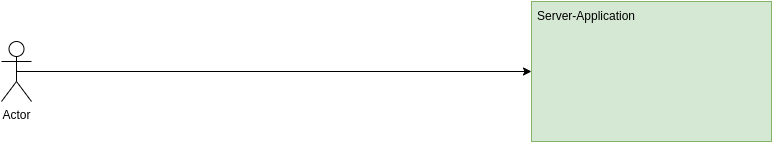
\includegraphics[width=10cm]{0_base.png}
\end{frame}

\begin{frame}{Warum ist OIDC? - Shared Secret}
\centering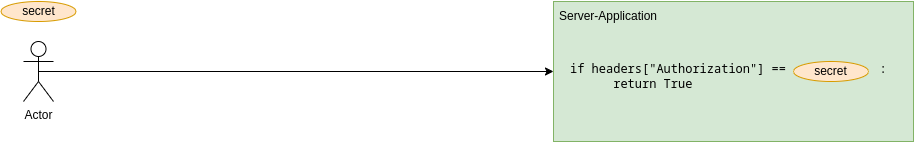
\includegraphics[width=10cm]{1_base_shared_secret.png}
\end{frame}

\begin{frame}{Warum ist OIDC? - HTTPS}
\centering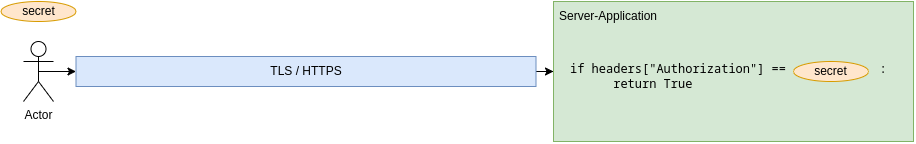
\includegraphics[width=10cm]{2_base_shared_secret_tls.png}
\end{frame}

\begin{frame}{Warum ist OIDC? - Just Salt}
\centering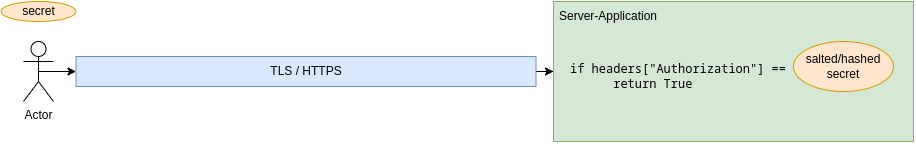
\includegraphics[width=10cm]{3_salted_hashed.png}
\end{frame}

\begin{frame}{Warum ist OIDC? - Just Salt}
\centering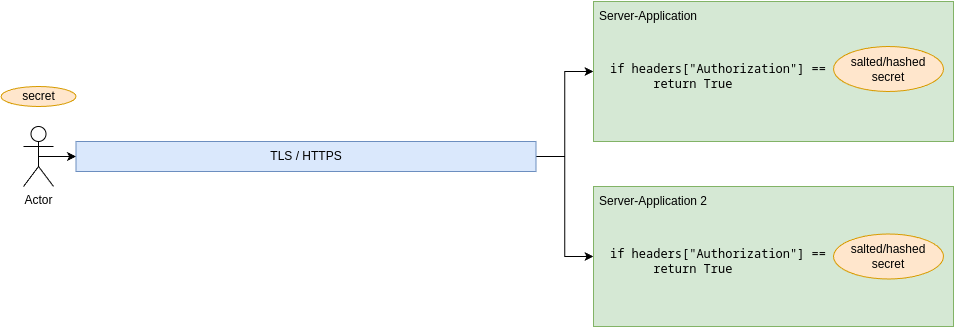
\includegraphics[width=10cm]{4_salted_multiple.png}
\end{frame}

\begin{frame}{Warum ist OIDC?}
\centering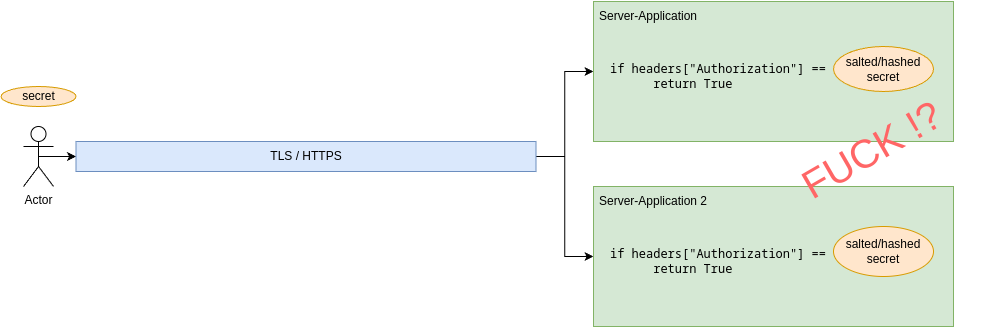
\includegraphics[width=10cm]{5_multiple_fuck.png}
\end{frame}

\begin{frame}{Warum ist OIDC? - LDAP}
\centering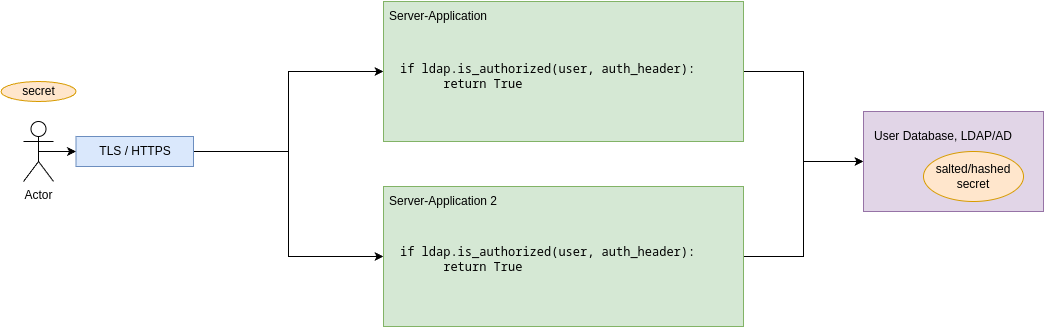
\includegraphics[width=10cm]{6_ldap_ad.png}
\end{frame}

\begin{frame}{Warum ist OIDC? - Trusted Gateway}
\centering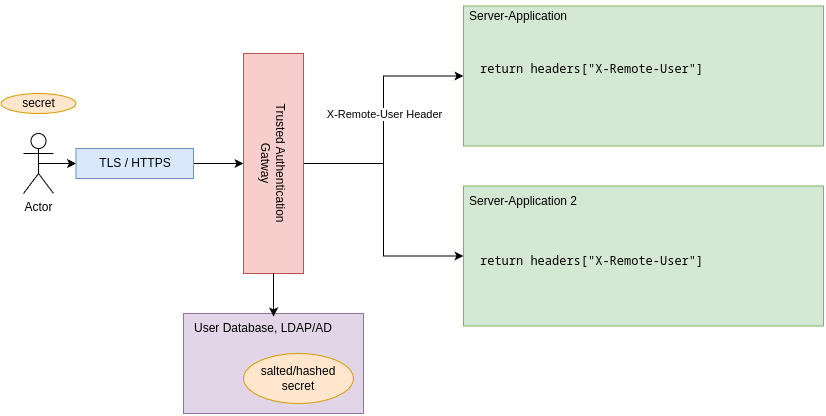
\includegraphics[width=10cm]{7_trusted_auth_gate.png}
\end{frame}

\begin{frame}{Warum ist OIDC? - Trusted Gateway}
\centering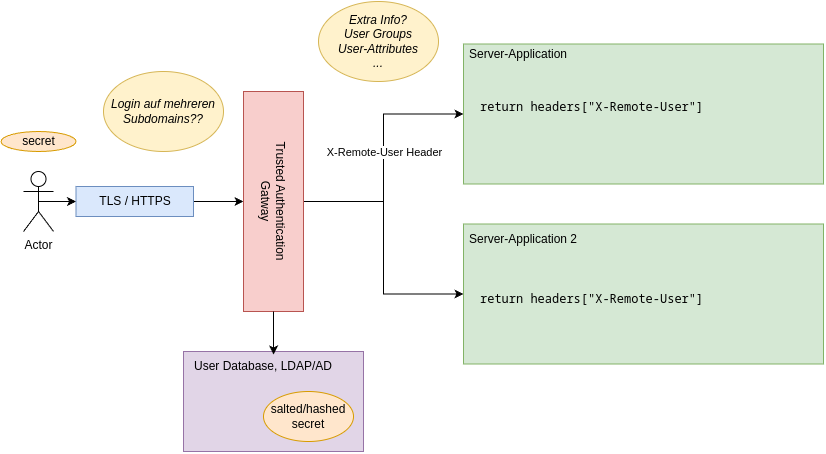
\includegraphics[width=10cm]{8_probleme_trusted_gate.png}
\end{frame}

\begin{frame}{Warum ist OIDC? - Menschen sind Affen}
\centering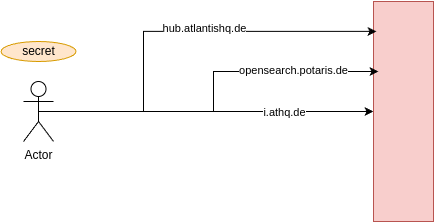
\includegraphics[width=10cm]{9_too_much_logins.png}
\end{frame}


\begin{frame}{Warum ist OIDC? - Menschen sind Affen}
\begin{tikzpicture}[remember picture,overlay]
    \node[anchor=north west, xshift=0cm, yshift=-2cm] at (current page.north west)
        {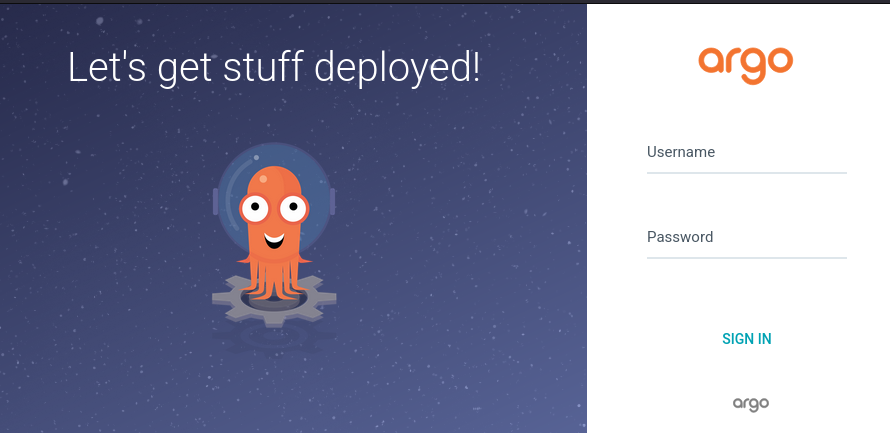
\includegraphics[width=8cm]{auth_argo.png}};
\end{tikzpicture}
\end{frame}


\begin{frame}{Warum ist OIDC? - Menschen sind Affen}
\begin{tikzpicture}[remember picture,overlay]
    \node[anchor=north west, xshift=0cm, yshift=-2cm] at (current page.north west)
        {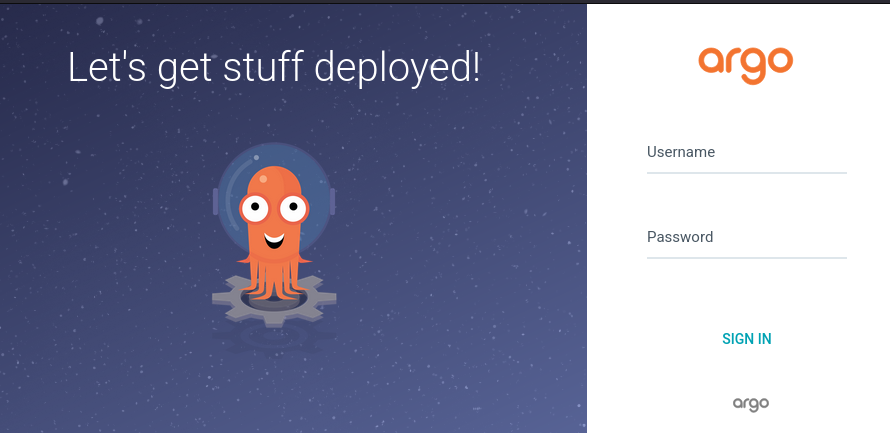
\includegraphics[width=8cm]{auth_argo.png}};
    \node[anchor=north east, xshift=0cm, yshift=-1cm] at (current page.north east)
        {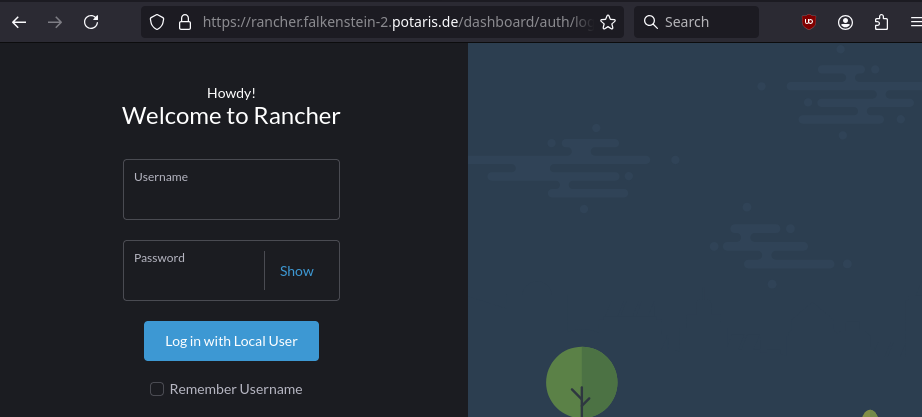
\includegraphics[width=8cm]{auth_rancher.png}};
\end{tikzpicture}
\end{frame}

\begin{frame}{Warum ist OIDC? - Menschen sind Affen}
\begin{tikzpicture}[remember picture,overlay]
    \node[anchor=north west, xshift=0cm, yshift=-2cm] at (current page.north west)
        {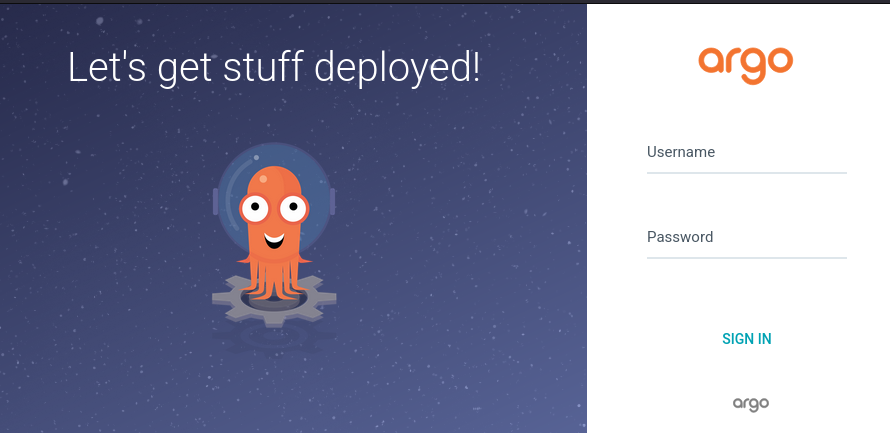
\includegraphics[width=8cm]{auth_argo.png}};
    \node[anchor=north east, xshift=0cm, yshift=-1cm] at (current page.north east)
        {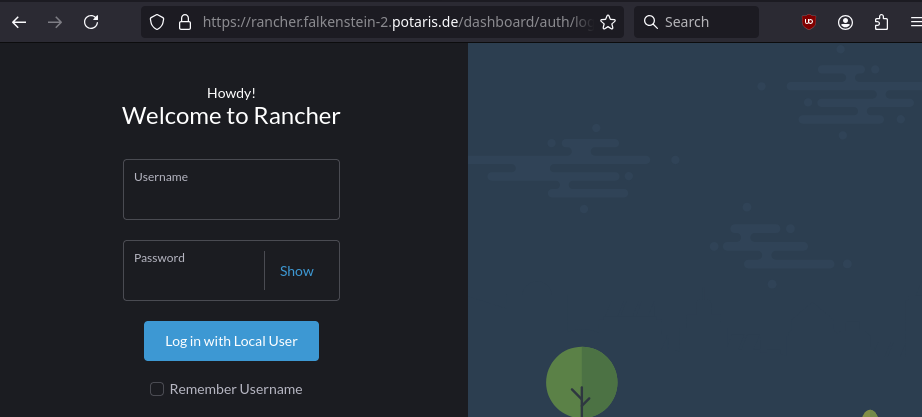
\includegraphics[width=8cm]{auth_rancher.png}};
    \node[anchor=south west, xshift=0cm, yshift=0cm] at (current page.south west)
        {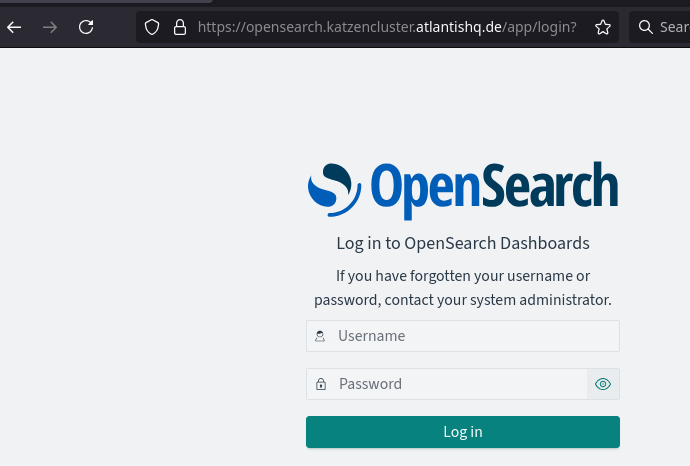
\includegraphics[width=8cm]{auth_opensearch.png}};
\end{tikzpicture}
\end{frame}

\begin{frame}{Warum ist OIDC? - Menschen sind Affen}
\begin{tikzpicture}[remember picture,overlay]
    \node[anchor=north west, xshift=0cm, yshift=-2cm] at (current page.north west)
        {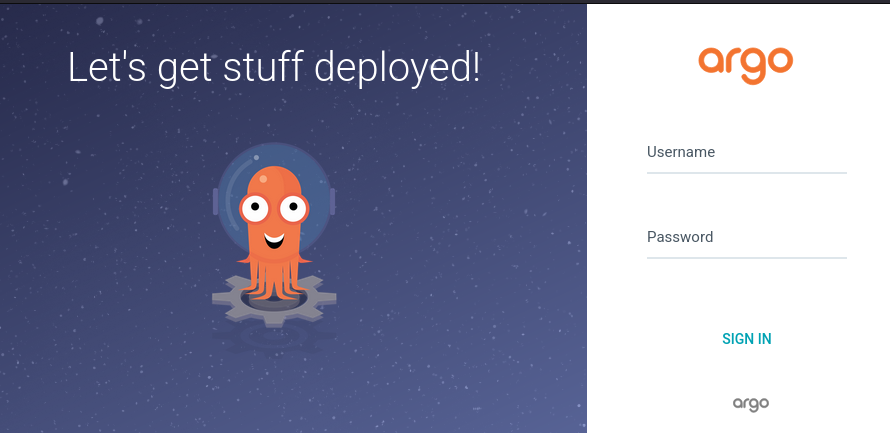
\includegraphics[width=8cm]{auth_argo.png}};
    \node[anchor=north east, xshift=0cm, yshift=-1cm] at (current page.north east)
        {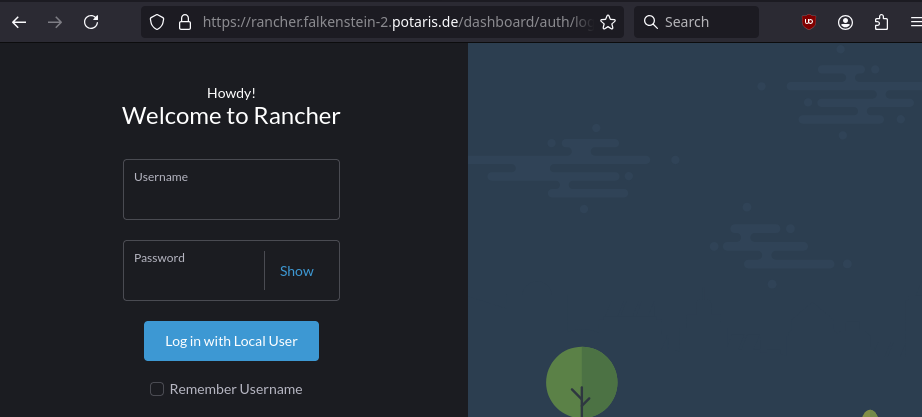
\includegraphics[width=8cm]{auth_rancher.png}};
    \node[anchor=south west, xshift=0cm, yshift=0cm] at (current page.south west)
        {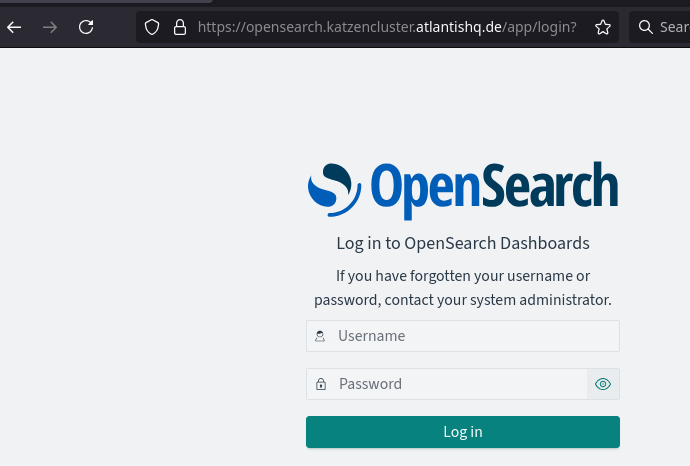
\includegraphics[width=8cm]{auth_opensearch.png}};
    \node[anchor=south east, xshift=0cm, yshift=0cm] at (current page.south east)
        {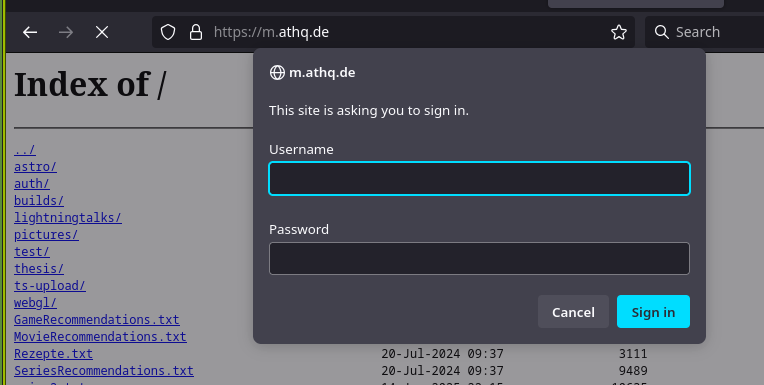
\includegraphics[width=8cm]{auth_basic_media.png}};
\end{tikzpicture}
\end{frame}

\begin{frame}{Warum ist OIDC?}
\centering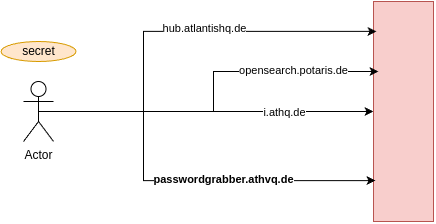
\includegraphics[width=10cm]{10_password_grabber.png}
\end{frame}

\begin{frame}{Was haben wir gelernt?}
\centering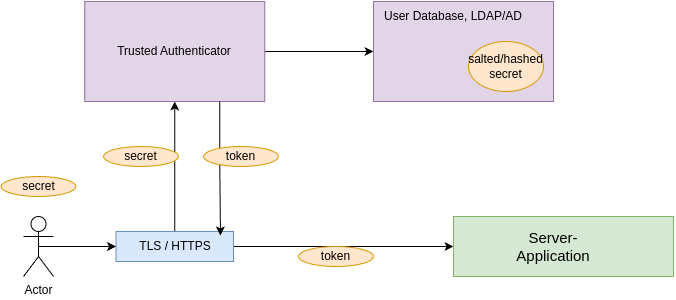
\includegraphics[width=10cm]{B_0_what_learned.drawio.png}
\end{frame}

%\begin{frame}{Lightning Talk Auth 9000}
%\centering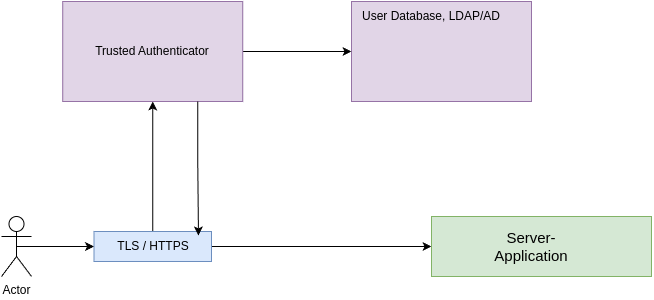
\includegraphics[width=10cm]{B_1_4_part_lets_name_it.png}
%\end{frame}

\begin{frame}{Lightning Talk Auth 9000}
\centering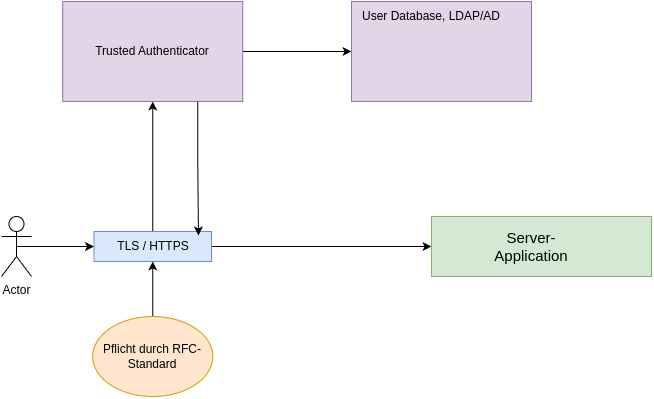
\includegraphics[width=10cm]{B_1_5_part_lets_name_it.png}
\end{frame}

\begin{frame}{Lightning Talk Auth 9000}
\centering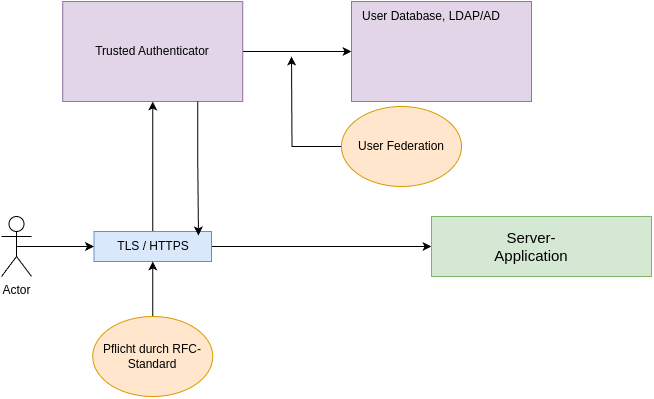
\includegraphics[width=10cm]{B_1_6_part_lets_name_it.png}
\end{frame}

\begin{frame}{Lightning Talk Auth 9000}
\centering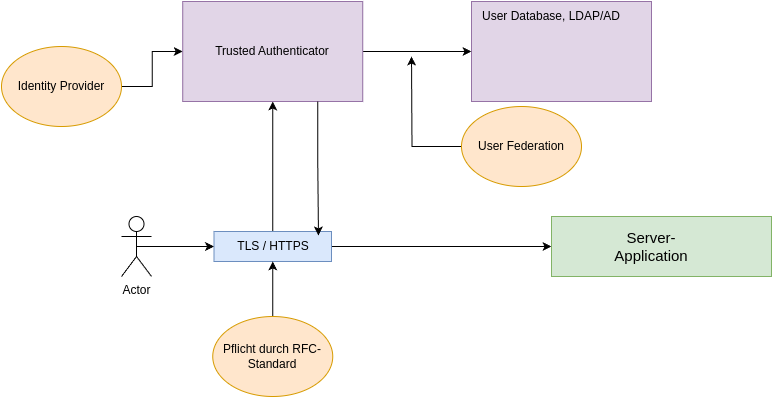
\includegraphics[width=10cm]{B_1_7_part_lets_name_it.png}
\end{frame}

\begin{frame}{Lightning Talk Auth 9000}
\centering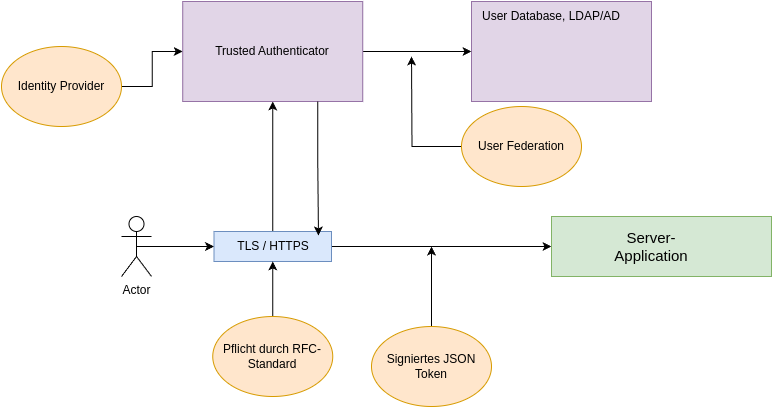
\includegraphics[width=10cm]{B_1_8_part_lets_name_it.png}
\end{frame}

\begin{frame}{Lightning Talk Auth 9000}
\centering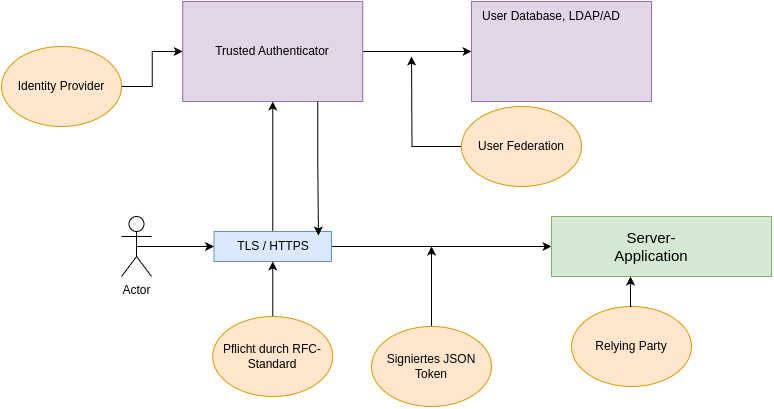
\includegraphics[width=10cm]{B_1_9_part_lets_name_it.png}
\end{frame}

\begin{frame}{Lightning Talk Auth 9000}
\centering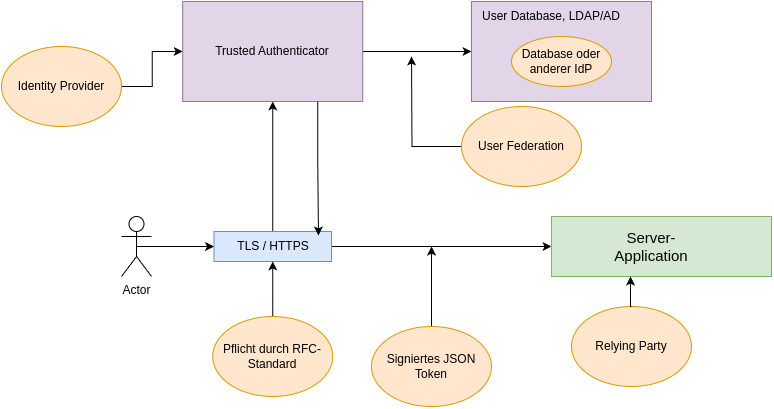
\includegraphics[width=10cm]{B_1_lets_name_it.png}
\end{frame}

\begin{frame}{OIDC}
\centering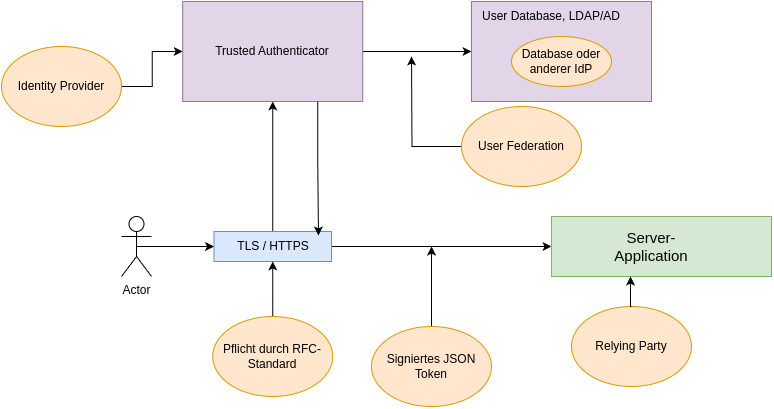
\includegraphics[width=10cm]{B_1_lets_name_it.png}
\end{frame}


\begin{frame}{OIDC - mehr oder weniger}
\centering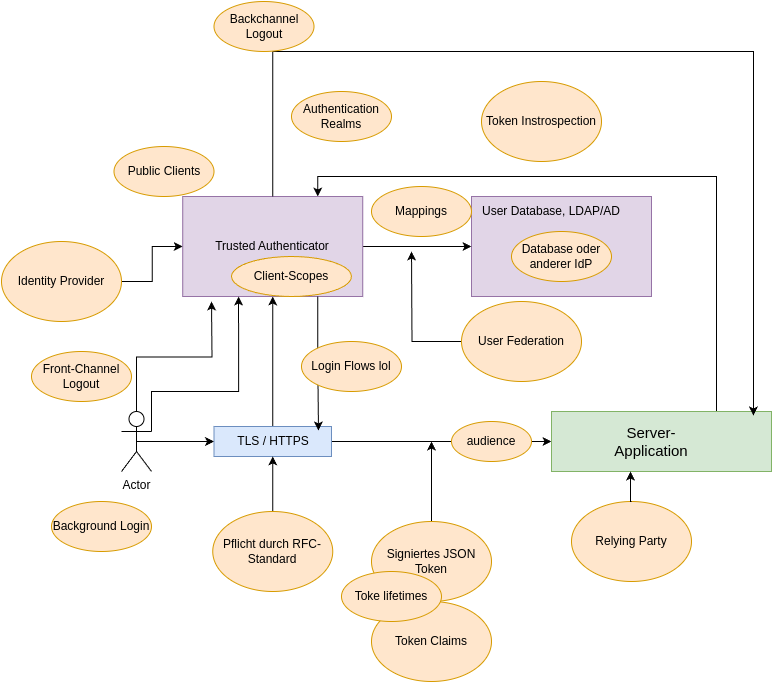
\includegraphics[width=9cm]{B_2_lets_name_it.png}
\end{frame}


\begin{frame}{Micro-Tutorial}
\centering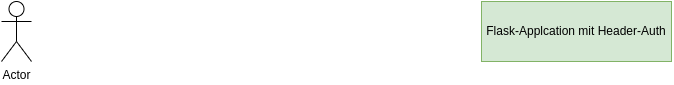
\includegraphics[width=9cm]{C_7_full_Keycloak_oatuh.png}
\end{frame}

\begin{frame}{Micro-Tutorial}
\centering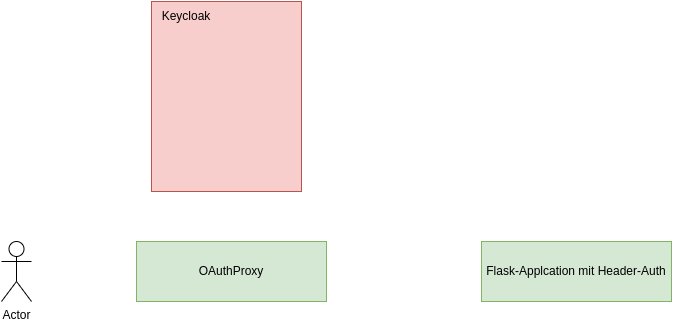
\includegraphics[width=9cm]{C_8_full_Keycloak_oatuh.png}
\end{frame}

\begin{frame}{Micro-Tutorial}
\centering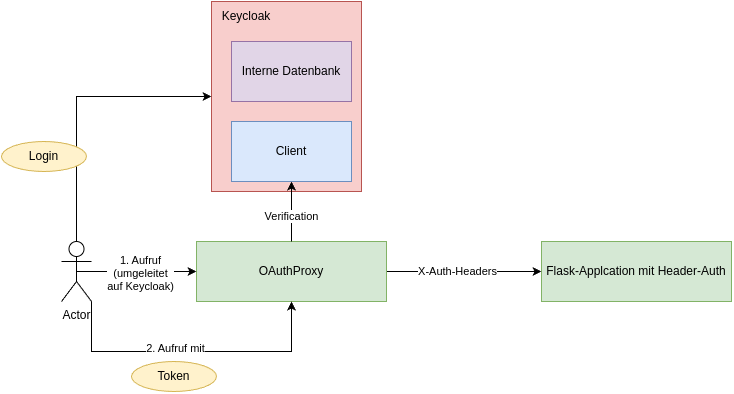
\includegraphics[width=9cm]{C_9_full_Keycloak_oatuh.png}
\end{frame}

%\begin{frame}[fragile]{Micro-Tutorial}
%\begin{lstlisting}
%docker run -p 8000:80
%    -e KC_BOOTSTRAP_ADMIN_PASSWORD=pw
%    keycloak:latest
%
%docker run -p 8080:8080
%	-e 
%    -e OAUTH2_PROXY_UPSTREAMS: http://localhost:5000/
%    -e OAUTH2_PROXY_CLIENT_ID: "client_name_here"
%    -e OAUTH2_PROXY_CLIENT_SECRET: "32-byte-secret"
%\end{lstlisting}
%\end{frame}

%\begin{frame}{Micro-Tutorial - Client}
%\hspace*{-1cm}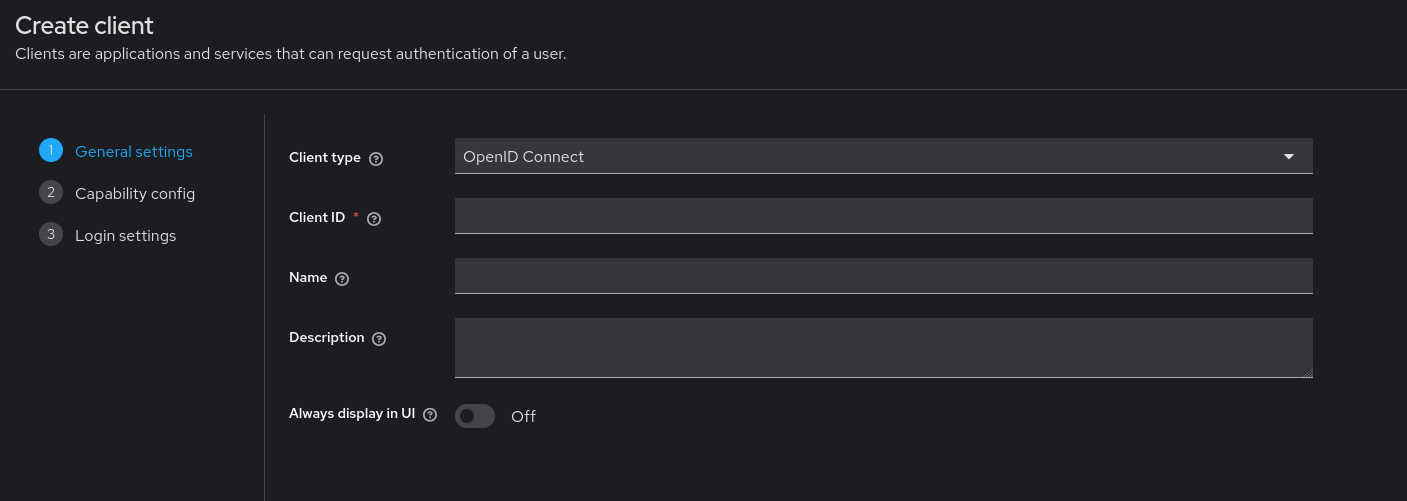
\includegraphics[width=13cm]{keycloak_client_1.png}
%\end{frame}

%\begin{frame}{Micro-Tutorial - Client}
%\hspace*{-1cm}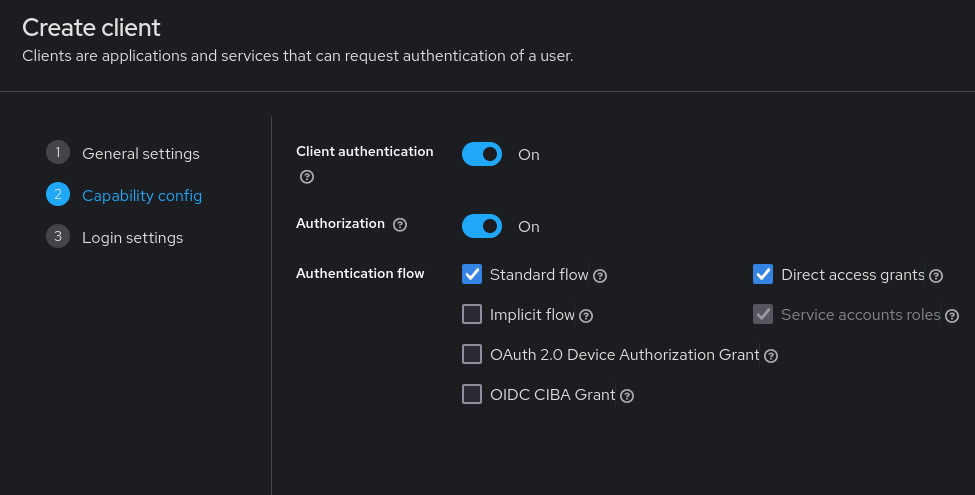
\includegraphics[width=13cm]{keycloak_client_2.png}
%\end{frame}

%\begin{frame}{Micro-Tutorial - Client}
%\hspace*{-1cm}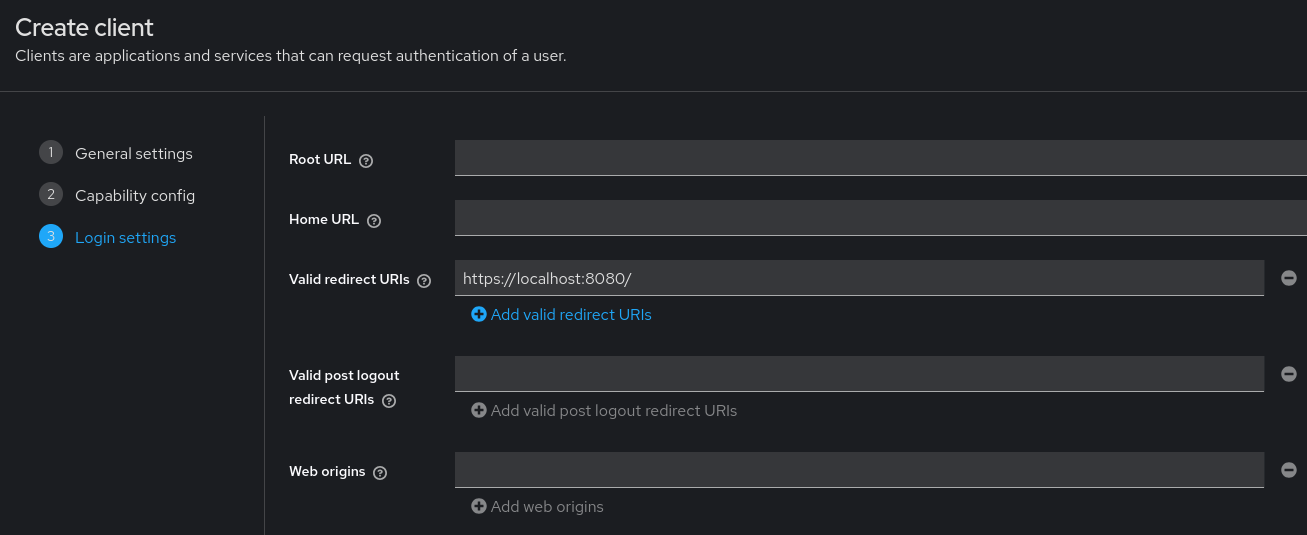
\includegraphics[width=13cm]{keycloak_client_3.png}
%\end{frame}

%\begin{frame}{Micro-Tutorial - Client}
%\hspace*{-1cm}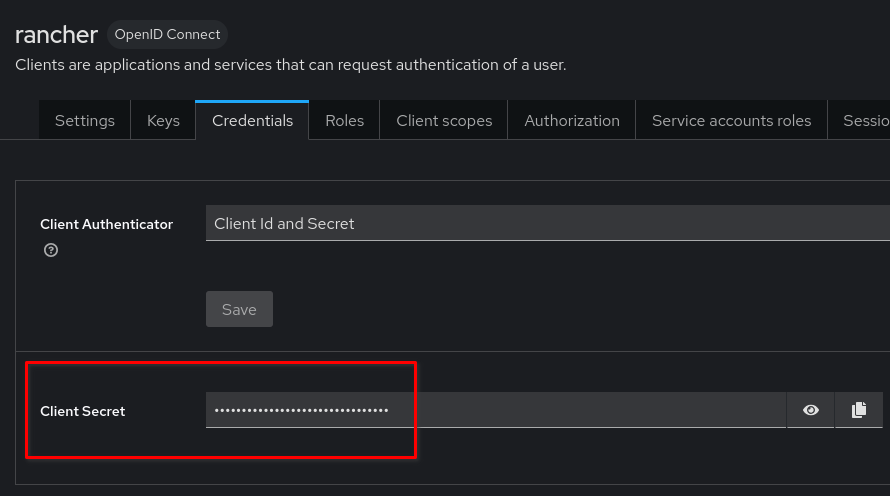
\includegraphics[width=13cm]{keycloak_client_4.png}
%\end{frame}

%\begin{frame}[fragile]{Micro-Tutorial}
%\begin{lstlisting}
%docker run -p 8000:80
%    -e KC_BOOTSTRAP_ADMIN_PASSWORD=pw
%    keycloak:latest

%docker run -p 8080:8080
%    -e OAUTH2_PROXY_UPSTREAMS: http://localhost:5000/
%    -e OAUTH2_PROXY_CLIENT_ID: "client_name_here"
%    -e OAUTH2_PROXY_CLIENT_SECRET: "<HERE>"
%\end{lstlisting}
%\end{frame}

\begin{frame}{Demonstration}
\href{https://hub.atlantishq.de}{\beamergotobutton{https://hub.atlantishq.de}}
\end{frame}

\begin{frame}{Fragen? Nächster Vortrag: Haskell to Hardware!}
\begin{itemize}
\item \textbf{Tutorial Basics}: potaris.de/posts/keycloak\_ansible/
\item \textbf{Tutorial Advanced}: potaris.de/posts/keycloak\_ldap\_1/
\item \textbf{Nächster Vortrag}: \textit{Clash - from Haskell to Hardware}
\item \textbf{Fragen}\\
\hspace*{5cm}
\includegraphics[width=3cm]{qr_code.png}
\end{itemize}
\end{frame}

\end{document}
